\documentclass[12pt, twoside]{article}
\usepackage[letterpaper, margin=1in, headsep=0.5in]{geometry}
\usepackage[english]{babel}
\usepackage[utf8]{inputenc}
\usepackage{amsmath}
\usepackage{amsfonts}
\usepackage{amssymb}
\usepackage{tikz}
%\usetikzlibrary{quotes, angles}

\usepackage{graphicx}
\usepackage{enumitem}
\usepackage{multicol}

\usepackage{fancyhdr}
\pagestyle{fancy}
\fancyhf{}
\renewcommand{\headrulewidth}{0pt} % disable the underline of the header

\fancyhead[LE]{\thepage}
\fancyhead[RO]{\thepage \\ Name: \hspace{4cm} \,\\}
\fancyhead[LO]{BECA / Dr. Huson / Geometry\\* Unit 6: Distance \& slope\\* 13 January 2019}

\begin{document}
\subsubsection*{7.8b Do Now: Exam followup}
  \begin{enumerate}

  \item Given isosceles $\triangle ABC$ with $\overline{AB} \cong \overline{BC}$, $m\angle B = 48$. Mark and label the diagram, and then find $m\angle A$. \hfill (\emph{the diagram is not to scale})
    \begin{flushright}
    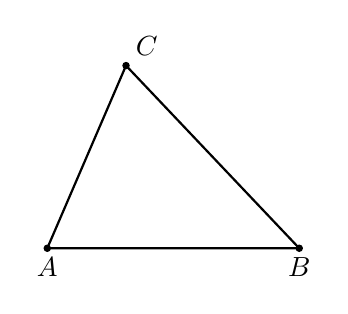
\begin{tikzpicture}[scale=0.8]
      \draw [thick](0,0)--(4,0)--(1.25,2.9)--(0,0);
      \draw [fill] (0,0) circle [radius=0.05] node[below]{$A$};
      \draw [fill] (4,0) circle [radius=0.05] node[below]{$B$};
      \draw [fill] (1.25,2.9) circle [radius=0.05] node[above right]{$C$};
    \end{tikzpicture}
    \end{flushright}
    
  \item The line $\overleftrightarrow{AB}$ has the equation $y=-\frac{2}{3}x+4$. Apply a dilation mapping $\overleftrightarrow{AB} \rightarrow \overleftrightarrow{A'B'}$ with a factor of $k=1.5$ centered at the origin. Draw and label the image on the grid. Write the equation of the line $\overleftrightarrow{A'B'}$.
    \begin{flushright} %4 quadrant regents grid w T-Chart
    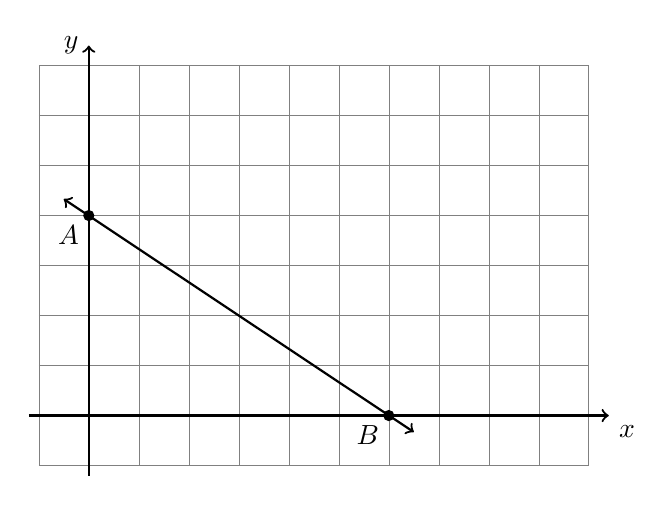
\begin{tikzpicture}[scale=.635]
      \draw [help lines] (-1,-1) grid (10,7);
      \draw [thick, ->] (-1.2,0) -- (10.4,0) node [below right] {$x$};
      \draw [thick, ->] (0,-1.2)--(0,7.4) node [left] {$y$};
      \draw [<->, thick] (-0.5,4.33)--(6.5,-0.33);
      \draw [fill] (0,4) circle [radius=0.1]node[below left]{$A$};
      \draw [fill] (6,0) circle [radius=0.1]node[below left]{$B$};
    \end{tikzpicture}
    \end{flushright}

    \item A triangle is dilated with factor $k$ such that $\triangle ABC \sim \triangle DEF$. Circle True or False.
    \begin{enumerate}[itemsep=0.5cm]
      \item T \quad F \quad $\angle A \cong \angle E$
      \item T \quad F \quad $\overline{AC} \cong \overline{DF}$
      \item T \quad F \quad $\displaystyle k=\frac{DF}{AC}$
      \item T \quad F \quad $\overline{AC} \rightarrow \overline{DF}$
      \item T \quad F \quad $\overline{AC} \cong \overline{DF}$
      \item T \quad F \quad $\displaystyle \frac{DE}{AB} = \frac{EF}{BC}$
    \end{enumerate}

\newpage
  \item Complete the construction of an equilateral triangle with one side as $\overline{XY}$. Show all construction marks, but make no extra lines. \vspace{3cm}
    \begin{center}
    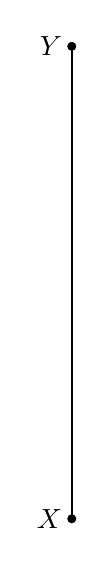
\begin{tikzpicture}
      \draw [-, thick] (0,0)--(0,6);
      \draw [fill] (0,0) circle [radius=0.05] node[left]{$X$};
      \draw [fill] (0,6) circle [radius=0.05] node[left]{$Y$};
    \end{tikzpicture}
    \end{center} \vspace{3cm}
    \begin{enumerate}
      \item Identify two circles in the construction. For each, name the center of the circle and the radius.  \vspace{3cm}
      \item Assuming that the third vertex of the triangle is point $Z$, explain why the distance from $X$ to $Z$ is the same as the distance from $X$ to $Y$.
    \end{enumerate}


\end{enumerate}
\end{document}